\subsection{Measurement apparatus}
\label{sec:meas-appar}
Figure~\ref{fig:exp_setup} shows a schematic view of the setup used for the
calibration of the detector and data taking. The signal from the detector at
first pass trough a pre-amplifier, this has a capacitance of 1~pF and is
connected to a high voltage power supply (HVPS) and to a pulse generator so that
the input voltage is directly proportional to the charge generated in the
detector through the well know formula\autocite{Knoll:RadMeasurement}
\begin{equation}
  \label{eq:capacitance}
  Q = CV.
\end{equation}
The pre-amplifier is then connected to a spectrum amplifier with adjustable
gain. From the spectrum amplifier the signal was sent to an oscilloscope for
online monitoring and adjustments and to a multi-channel analyzer (MCA) that was
connected to a computer to record the data.
\begin{figure}[!h]
  \centering
  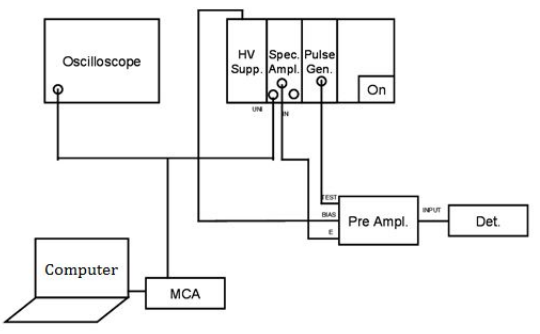
\includegraphics[width=.5\linewidth]{experimental_setup}
  \caption{Schema of the experimental setup}
  \label{fig:exp_setup}
\end{figure}

\subsection{Calibration}
\label{sec:calibration}
In order to calibrate the detector the pulse generator was used to injected in
the pre-amplifier a known pulse. The oscilloscope was used to read the pulse
voltage that multiplied by the pre-amplifier capacitance gives the collected
charge as described in Section~\ref{sec:meas-appar}. The distribution on the MCA
was fitted with a Gaussian using the data taking software, the mean value is
then associated to a charge and the standard deviation used as uncertainty. This
procedure was performed for a set of input voltages and, due to time
restrictions, only for a gain value of 100. Figure~\ref{fig:calibration_fit}
shows the calculated collected charge as a function of the MCA channel number
with a linear fit superimposed. Figure~\ref{fig:calibration_raw} shows the
counts as a function of the MCA channel number.
\begin{figure}[!h]
  \centering
  \begin{subfigure}[t]{.48\linewidth}
    \includegraphics[width=\linewidth]{calibration_fit}
    \caption{Collected charge as a function of the multi-channel number}
    \label{fig:calibration_fit}
  \end{subfigure}
  \begin{subfigure}[t]{.48\linewidth}
    \includegraphics[width=\linewidth]{calibration_raw}
    \caption{Counts as a function of the multi-channel number}
    \label{fig:calibration_raw}
  \end{subfigure}
  \caption{}
  \label{fig:calibration}
\end{figure}
%%% Local Variables:
%%% mode: latex
%%% TeX-master: "prop_counter"
%%% End:
